\documentclass[conference]{IEEEtran}
\usepackage{times}
\usepackage{algorithm}
\usepackage{algpseudocode}
\usepackage{subfigure}
\usepackage{graphicx}
\usepackage{subfloat}
\usepackage{float}
\usepackage{amsmath,empheq}
\usepackage{amssymb}
\usepackage{latexsym}

\usepackage[numbers]{natbib}
\usepackage{multicol}
\usepackage[bookmarks=true]{hyperref}
\usepackage[usenames,dvipsnames]{color}

% -- Comment commands --
\newcommand{\stnote}[1]{\textcolor{Blue}{\textbf{ST: #1}}}
\newcommand{\dnote}[1]{\textcolor{Green}{\textbf{D: #1}}}

\pdfinfo{
   /Author (David Abel  \& Gabriel Barth-Maron, James MacGlashan, Stefanie Tellex)
   /Title  (Toward Affordance-Aware Planning)
   /CreationDate (D:20101201120000)
   /Subject (Planning, Affordances, Sequential Decision Making)
   /Keywords (Planning, Affordance, MDP, Learning)
}

\begin{document}

% paper title
\title{Affordance-Aware Planning}

% Author info:
\author{\authorblockN{David Abel \& Gabriel Barth-Maron, James MacGlashan, Stefanie Tellex}
\authorblockA{Department of Computer Science, Brown University \\
\texttt{\{dabel,gabrielbm,jmacglashan,stefie10\}@cs.brown.edu}}}

\maketitle

\begin{abstract}
Planning algorithms for non-deterministic domains are often
intractable in large state spaces due to the well-known ``curse of
dimensionality.''  Existing approaches to address this problem fail to prevent autonomous agents
from considering many actions which would be obviously irrelevant to a
human solving the same problem. We formalize the notion of affordances
as knowledge added to an MDP that prunes actions in a state- and
reward- general way. This pruning significantly reduces the number of
state-action pairs the agent needs to evaluate in order to act
optimally. We demonstrate our approach in the Minecraft domain as a
model for robotic tasks, showing significant increase in speed and
reduction in state-space exploration during planning. Further, we
provide a learning framework that enables an agent to learn
affordances through experience, opening the door for agents to learn
to adapt and plan through new situations. We provide preliminary
results indicating that the learning process effectively produces
affordances that help solve an MDP faster, suggesting that affordances
serve as an effective, transferable piece of knowledge for planning
agents in large state spaces. We compare our approach with several
existing knowledge engineering methods and deploy an affordance-aware planner
on ReThink's Baxter as part of a cooperative cooking task.

\end{abstract}

\IEEEpeerreviewmaketitle

% ====== Section: Introduction ======
\section{Introduction}
\label{sec:introduction}

As robots move out of the lab and into the real world, planning
algorithms need to scale to domains of increased noise, size, and
complexity.  A classic formalization of this problem is a stochastic
sequential decision making problem in which the agent must find a
policy (a mapping from states to actions) for some subset of the state
space that enables the agent to achieve a goal from some initial
state, while minimizing any costs along the way.
Increases in planning problem size and complexity directly correspond
to an explosion in the state-action space, restricting extensions to large state-spaces
such as robotic applications. Current approaches to solving 
sequential decision making problems in the face of uncertainty cannot tackle these problems 
as the state-action space becomes too large~\cite{grounds05}.

To address this state-space explosion, prior work has explored adding
knowledge to the planner to solve problems in these
massive domains, such as options~\cite{sutton99} and
macroactions~\cite{Botea:2005kx,Newton:2005vn}. However, these
approaches add knowledge in the form of additional high-level actions
to the agent, which {\em increases} the size of the state-action space
(while also allowing the agent to search more deeply within the
space).  The resulting augmented space is even larger, which can have
the paradoxical effect of increasing the search time for a good
policy~\cite{Jong:2008zr}. Other approaches fall short of learning useful, transferable knowledge,
either due to complexity or lack of generalizability.

Instead, we propose a formalization of {\em affordances} \cite{gibson77} for Markov Decision Processes (MDPs) that
specifies which actions an agent should consider in different kinds of states to achieve a certain kind of goal.
Our approach enables an agent to focus on
aspects of the environment that are most relevant toward solving its current goal 
and avoids exploration of irrelevant parts of the 
state-action space, which leads to dramatic speedups in planning.

Further, we created a learning process that enables agents to
autonomously learn affordances through experience, lessening the
agent's dependence on expert knowledge. Affordances are not specific
to a particular reward function or state space, and provide the agent
with transferable knowledge that is effective in a wide variety of
problems. We call any planner that uses affordances an {\it
  affordance-aware} planner.

Because affordances define the {\em kind} of goals for which actions
are useful, affordances also enable high-level reasoning that can be
combined with approaches like subgoal planning for even
greater performance gains. In our current model, ideal subgoals are
sometimes given directly to planning agents by an expert - however, we are
interested in automatically discovering subgoals in an online way, a
problem which has already enjoyed some success
\cite{Mcgovern01automaticdiscovery,Simsek:2005:IUS:1102351.1102454}.


% ====== Section: Background ======
\section{Background}
\label{sec:background}

We use Minecraft as our planning and evaluation domain. Minecraft is a
3-D blocks world game in which the user can place and destroy blocks
of different types.   It serves as a model for a variety of robotic tasks involving assembly and construction.  Minecraft's physics and action space are expressive
enough to allow very complex systems to be created by users, including logic gates and 
functional scientific graphing calculators\footnote{https://www.youtube.com/watch?v=wgJfVRhotlQ};
simple scenes from a Minecraft world appear in Figure~\ref{fig:epicworld} - a video demonstration of
an early iteration of an affordance-aware planner solving this task may be seen online\footnote{Watch at: https://vimeo.com/88689171}.
Minecraft serves as a model for robotic tasks such as cooking assistance, assembling items in a factory, 
and object retrieval.  As in these tasks, the agent operates in a very large state-action space in an uncertain environment.

\begin{figure*}
\centering
\subfigure[Start]{
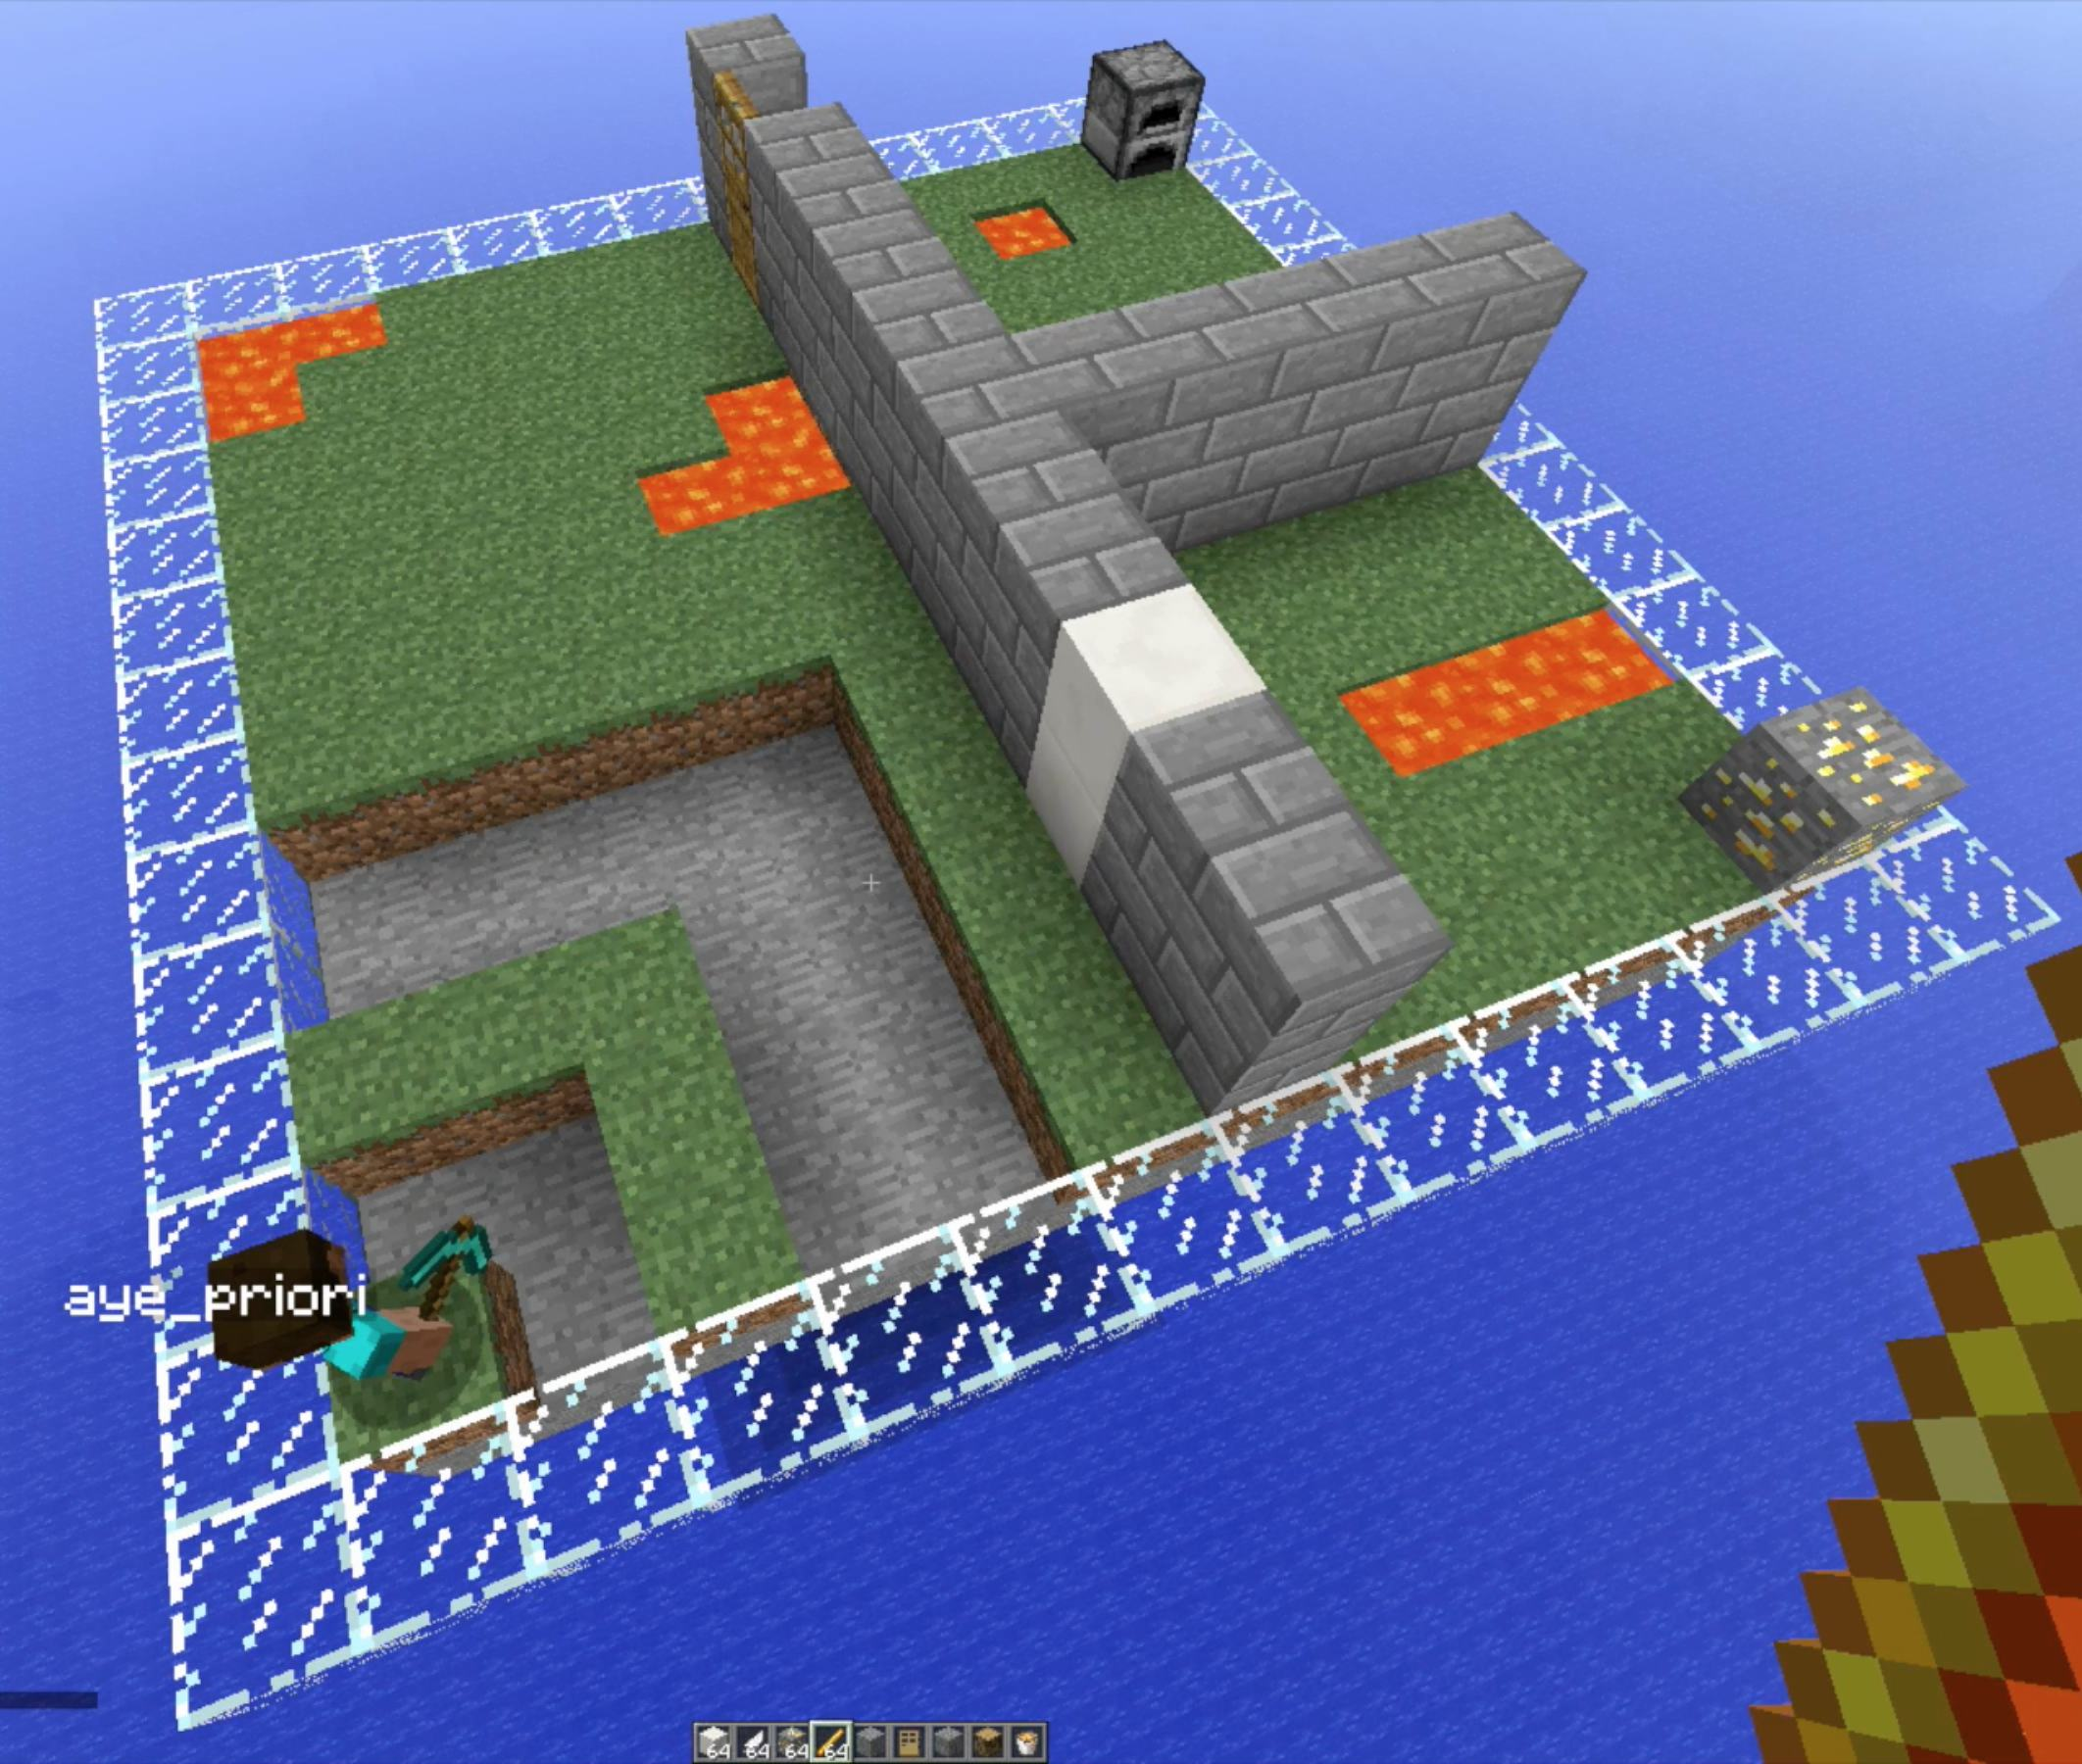
\includegraphics[width=0.23\linewidth]{figures/epicworld_1.jpg}}%
\subfigure[Destroy Wall]{
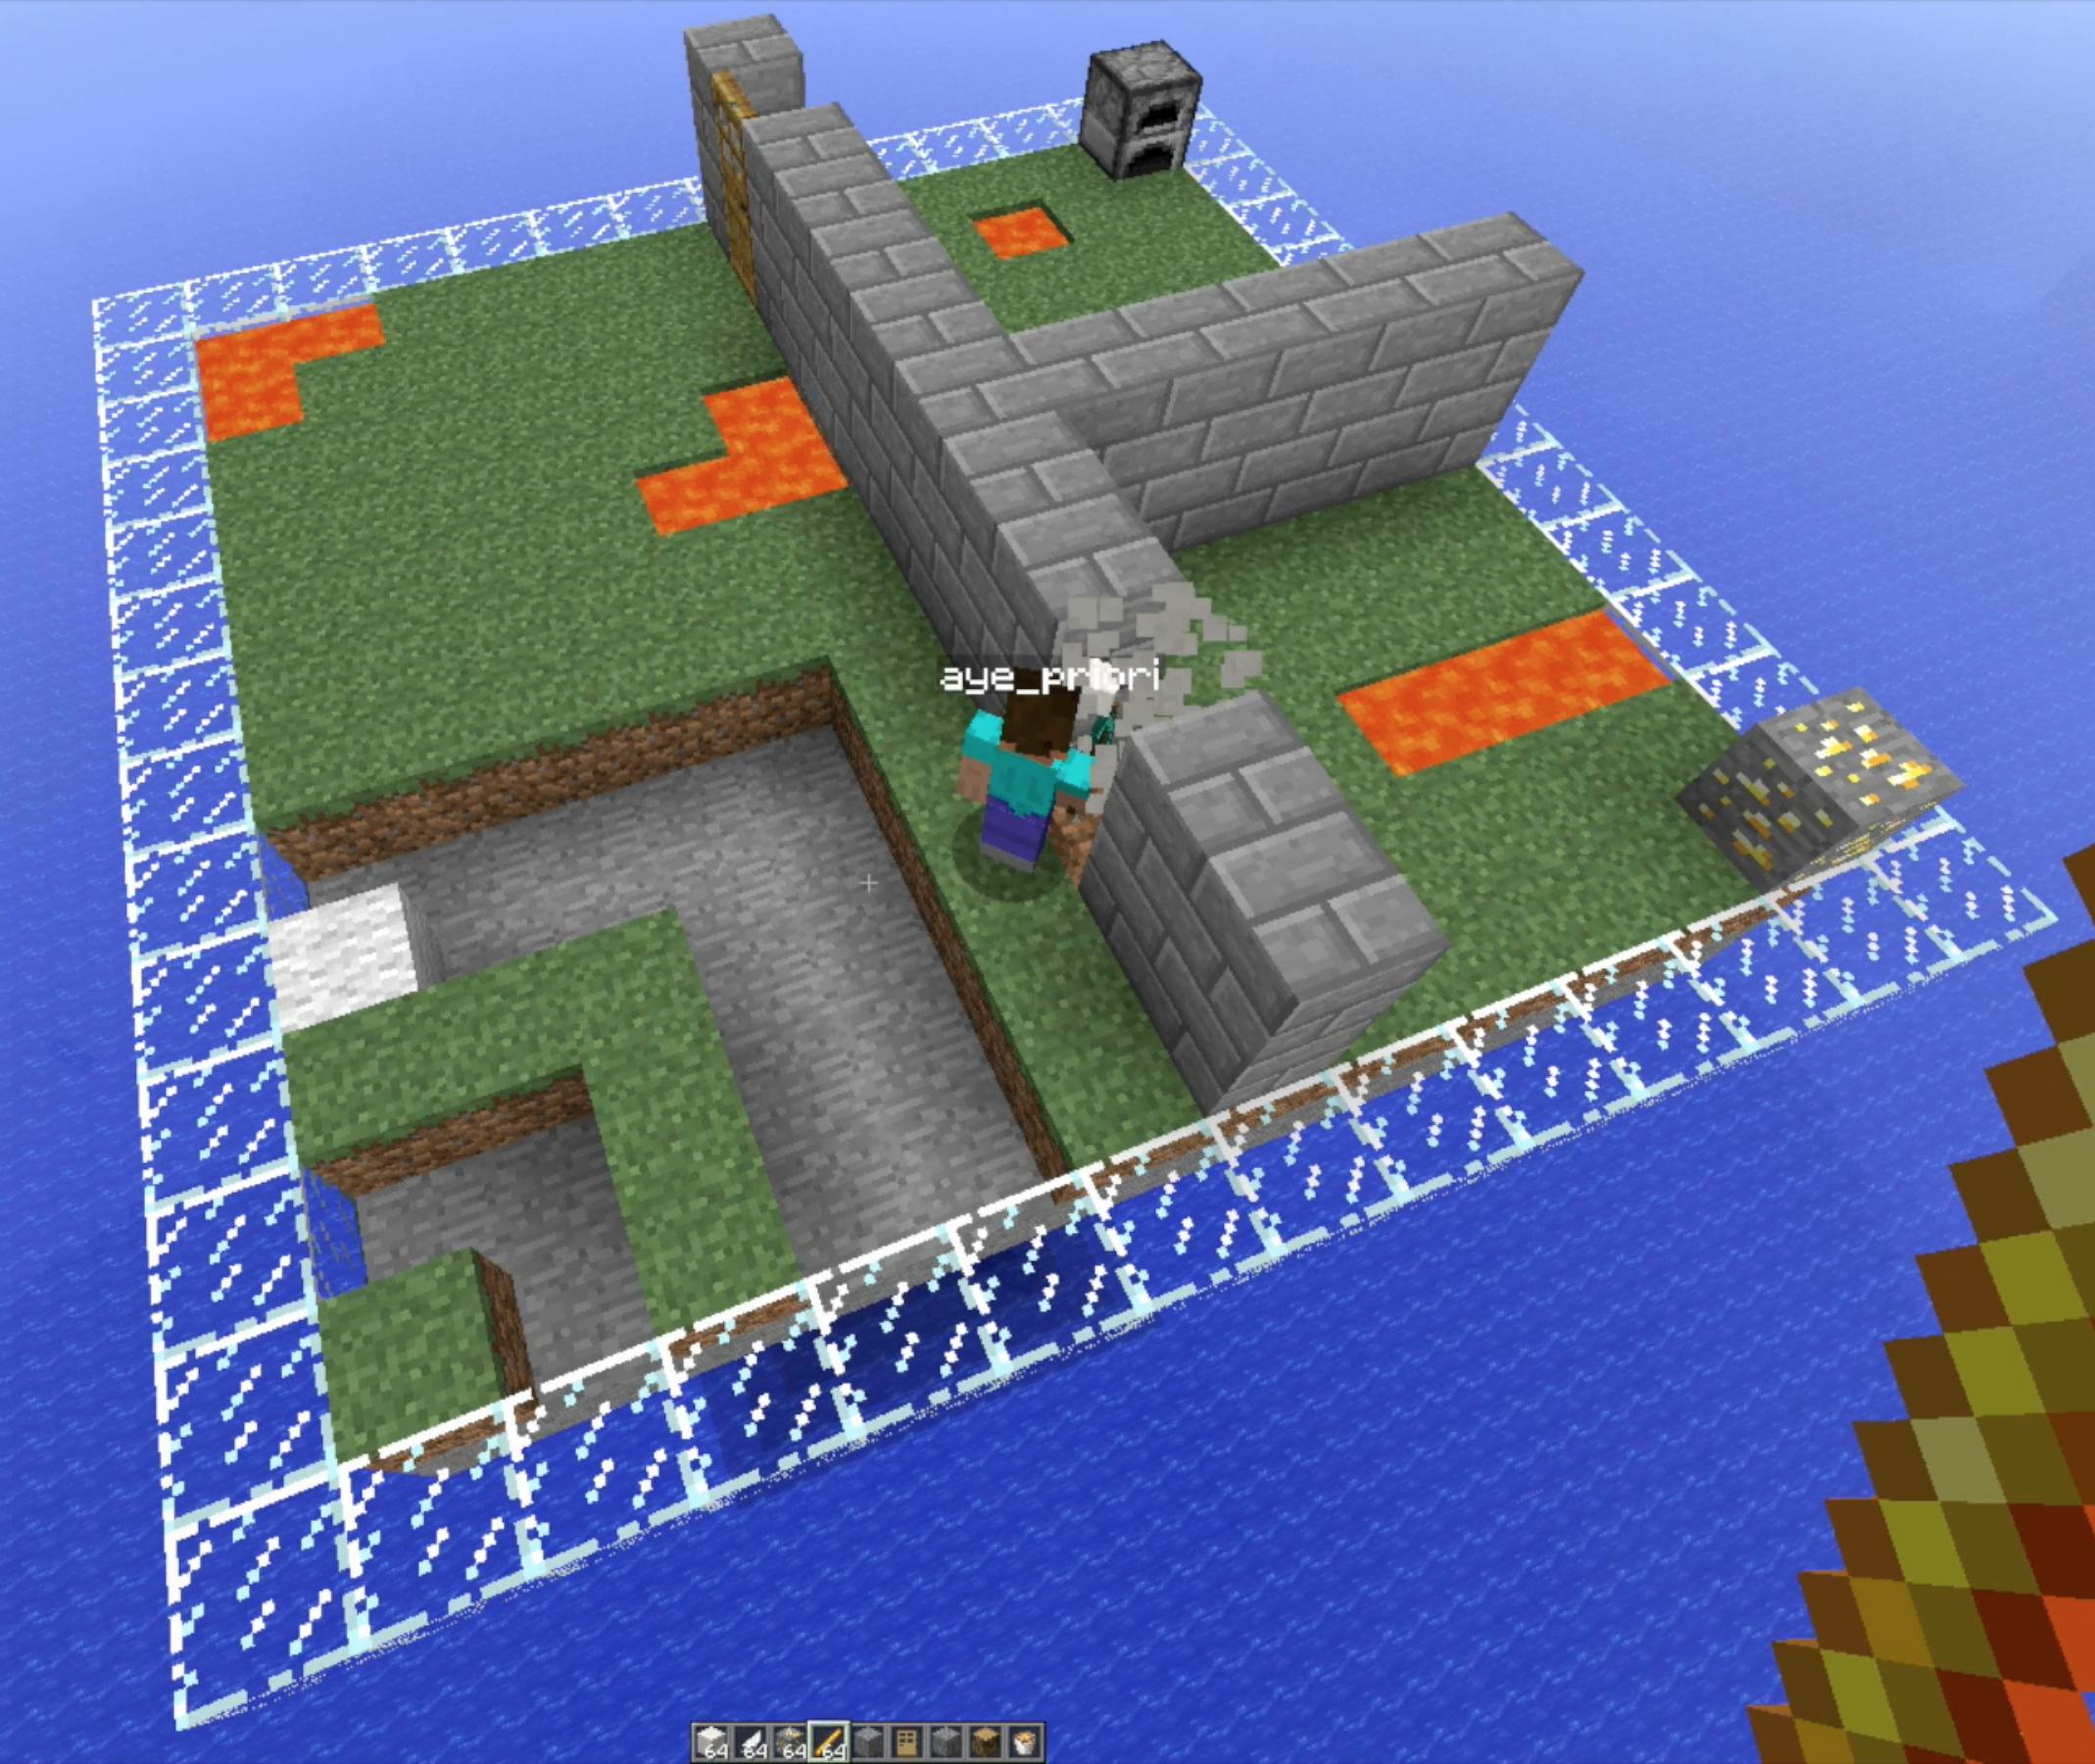
\includegraphics[width=0.23\linewidth]{figures/epicworld_2.jpg}}%
\subfigure[Collect Ore]{
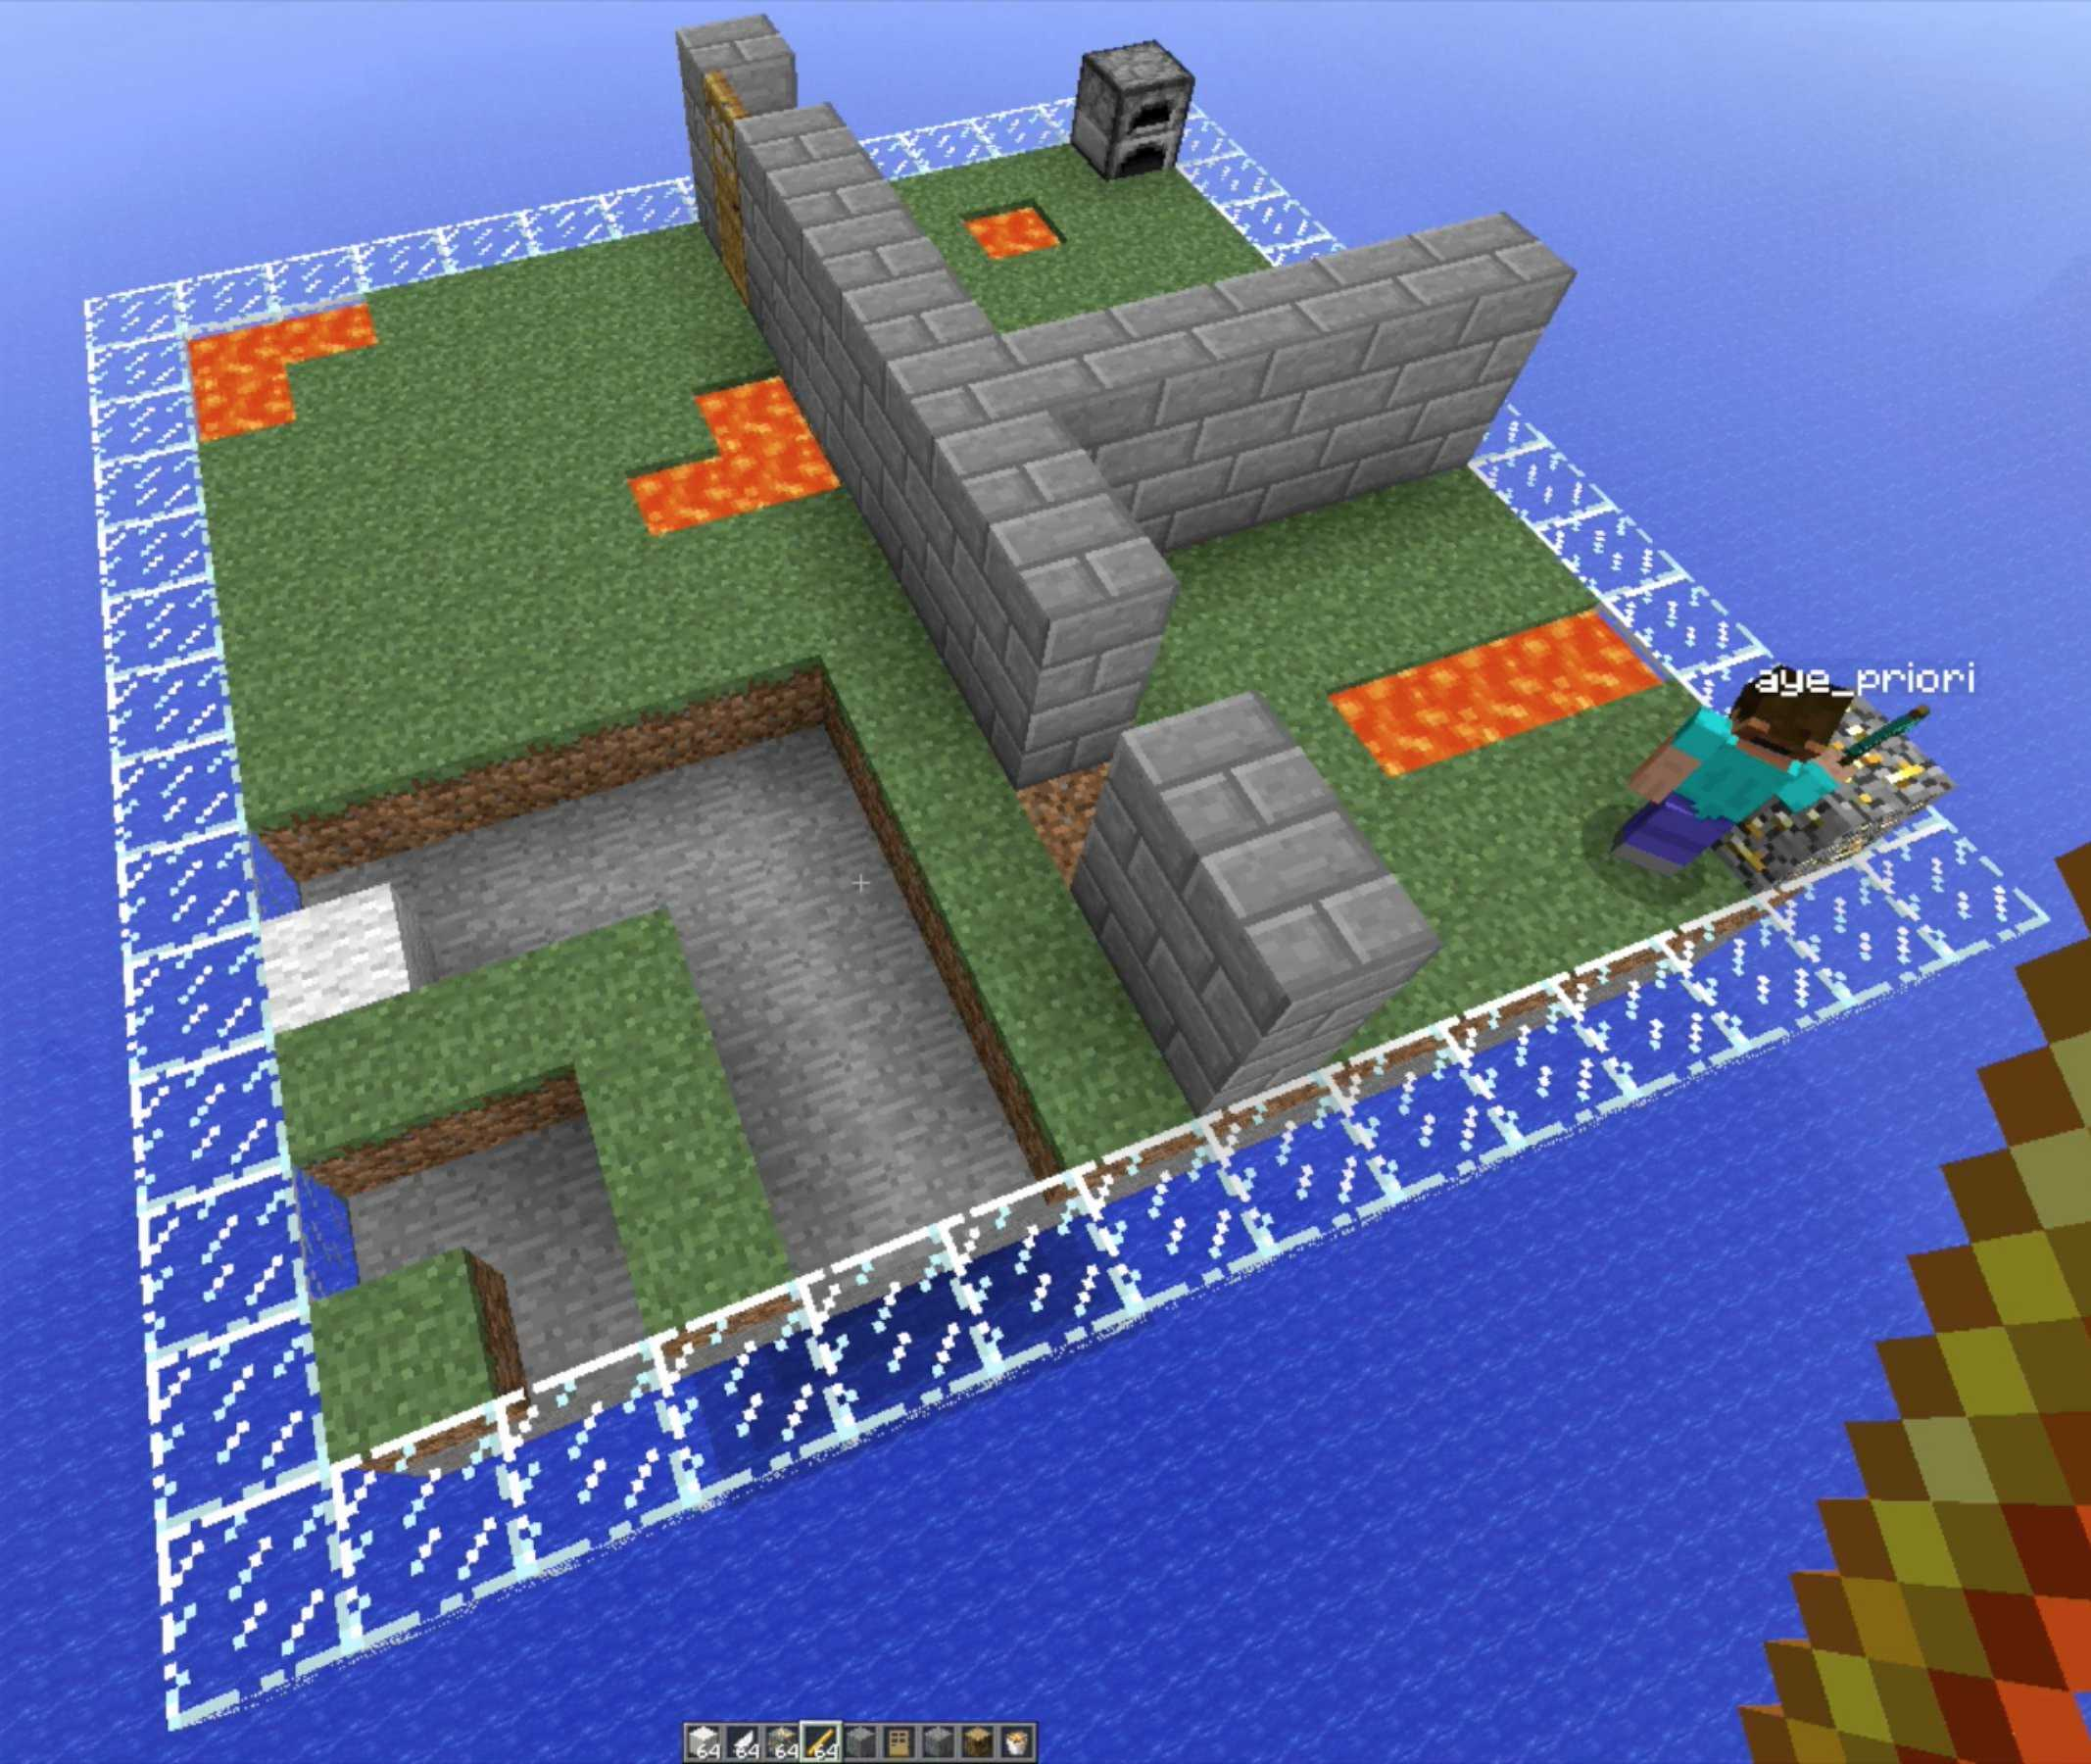
\includegraphics[width=0.23\linewidth]{figures/epicworld_3.jpg}}%
\subfigure[Smelt Ore]{
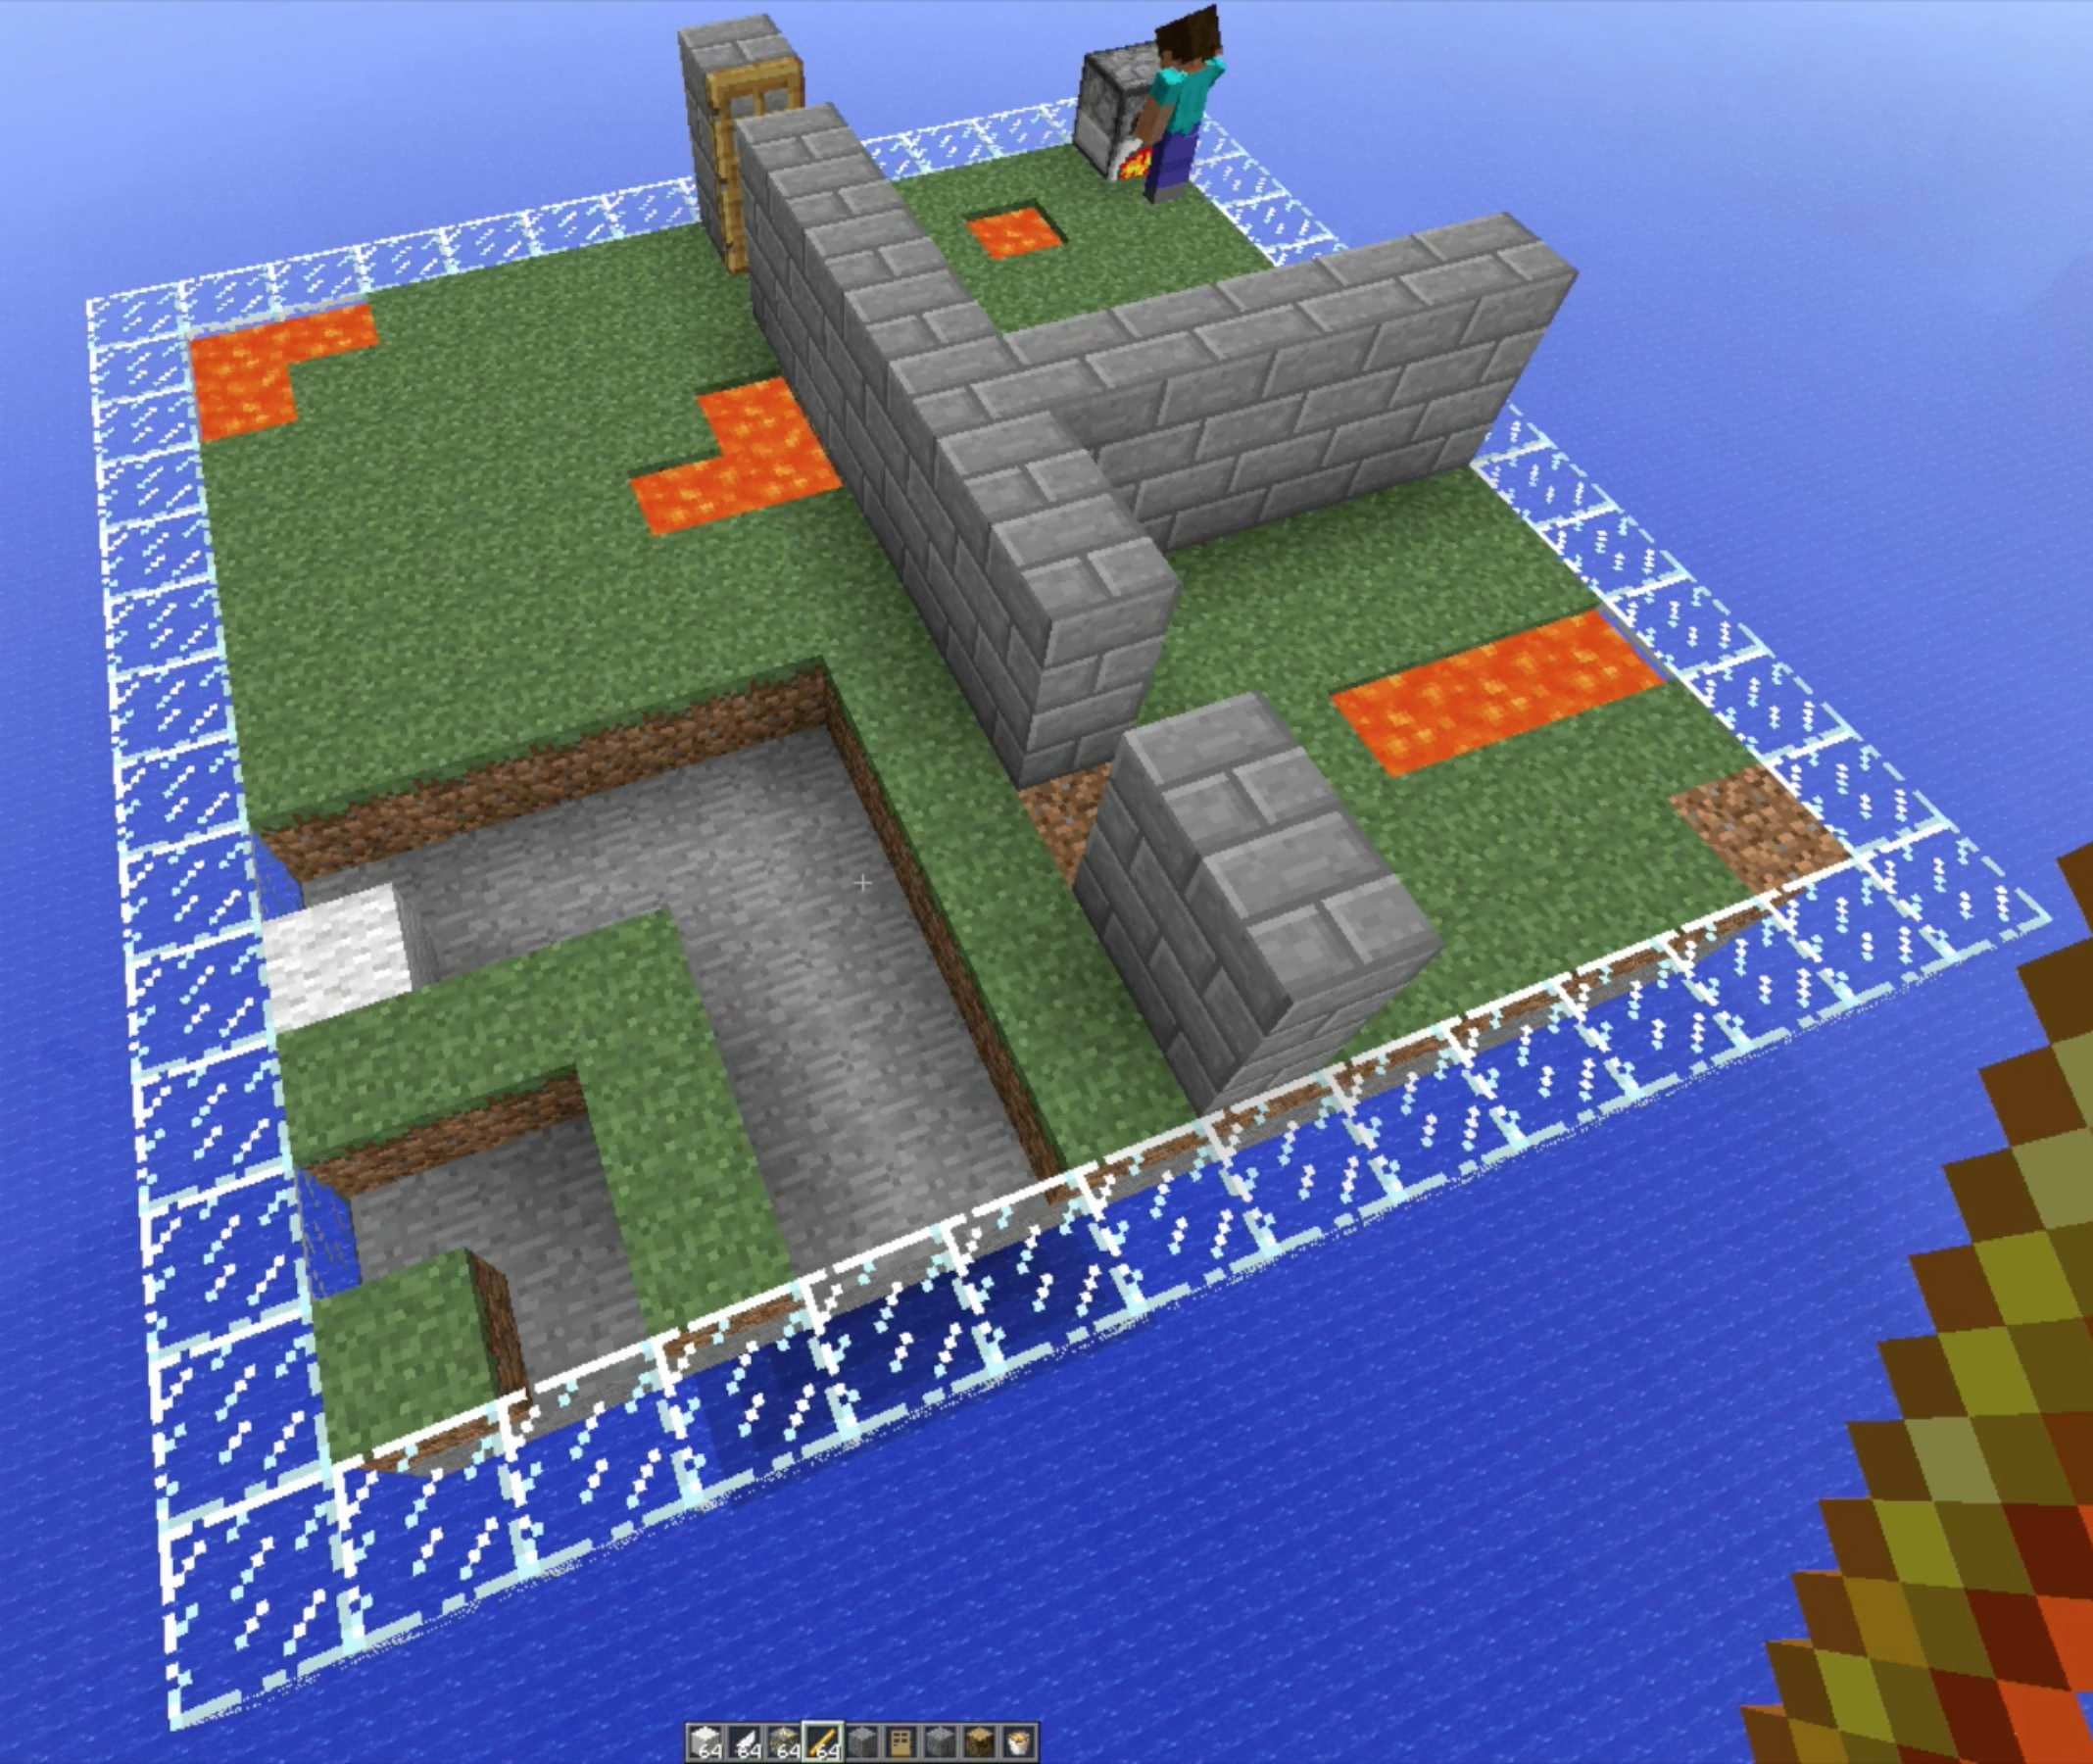
\includegraphics[width=0.23\linewidth]{figures/epicworld_4.jpg}}%
  \caption{Affordance-aware RTDP tasked with a gold-smelting task with a variety of obstacles
  (only solved by an affordance-aware planner)}
  \label{fig:epicworld}
\end{figure*}

Minecraft is also an effective parallel for the actual world, both
in terms of approximating the complexity and scope of planning
problems, as well as modeling the uncertainty and noise presented to a
robotic agent.  For instance, robotic agents are prone to
uncertainty throughout their system, including noise in their
sensors (cameras, LIDAR, microphones, etc.), odometry, control, and
actuation.  In order to accurately capture some of the inherent
difficulties of planning under uncertainty, the Minecraft agent's
actions were modified to have stochastic outcomes. These stochastic
outcomes may require important changes in the optimal policy in
contrast to deterministic actions, such as keeping the agent's
distance from high cost areas of the state-space, such as lava or cliffs.

We chose to give the Minecraft agent perfect sensor data about the Minecraft world.
However, affordances typically relate to the agent's immediate surroundings,
so limiting the perceptual scope should not impede the performance gains of affordances.
We have considered extensions to Partially Observable domains, though at a distance
solving a POMDP is effectively unchanged by the presence of affordances (beyond the
performance gains provided by pruning actions).

\subsection{OO-MDPs}

We define affordances in terms of propositional functions on states. Our definition builds on the Object-Oriented Markov Decision Process
(OO-MDP) \cite{diuk08}.  OO-MDPs are an extension of
the classic Markov Decision Process (MDP).  A classic MDP is a
five-tuple: $\langle \mathcal{S}, \mathcal{A}, \mathcal{T},
\mathcal{R}, \gamma \rangle$, where $\mathcal{S}$ is a state-space;
$\mathcal{A}$ is the agent's set of actions; $\mathcal{T}$ denotes
$\mathcal{T}(s' \mid s,a)$, the transition probability of an agent
applying action $a \in \mathcal{A}$ in state $s \in \mathcal{S}$ and
arriving in $s' \in \mathcal{S}$; $\mathcal{R}(s,a,s')$ denotes the
reward received by the agent for applying action $a$ in state $s$ and
and transitioning to state $s'$; and $\gamma \in [0, 1)$ is a discount
  factor that defines how much the agent prefers immediate rewards
  over distant rewards (the agent more greatly prefers to maximize
  more immediate rewards as $\gamma$ decreases).

A classic way to provide a factored representation of an MDP state is to represent
each MDP state as a single feature vector. By contrast, an OO-MDP represents the state space as a collection of objects,
$O = \{o_1, \ldots, o_o \}$.  Each object $o_i$ belongs to a
class $c_j \in  \{c_1, \ldots, c_c\}$. Every class has a set of attributes
$Att(c) = \{c.a_1, \ldots, c.a_a \}$, each of which has a domain $Dom(c.a)$ of possible values.
Upon instantiation of an object class, its attributes are given a state $o.state$
(an assignment of values to its attributes).  The underlying MDP state is the set
of all the object states: $s \in {\cal S} = \cup_{i = 1}^o \{o_i.state\}$. 

Our motivation for using an OO-MDP lies in the ability to
formulate predicates over classes of objects. That is, the OO-MDP
definition also includes a set of predicates ${\cal P}$ that operate
on the state of objects to provide additional high-level information
about the MDP state. 

While an OO-MDP reduces the size of the Minecraft state space
by a significant factor, the resulting state space is still far too large to
solve with any existing (OO)-MDP solver. This is the primary motivator
for incorporating affordances - to reduce the amount of the
state space that an OO-MDP agent will have to explore.

The Brown UMBC Reinforcement Learning And Planning framework (BURLAP\footnote{http://burlap.cs.brown.edu/})
is working toward integrating planning and reinforcement learning algorithms with a variety of planning domains represented
as an OO-MDP, including ROS. In this way, transferable knowledge like affordances can be quickly deployed
to domains like Mountain Car \cite{Moore90efficientmemory-based} and Minecraft, but also to a variety
of Robots that utilize ROS. Our group is also working to deploy affordances as a
means of knowledge representation and reasoning for collaborative cooking with ReThink's Baxter.

% ====== Section: Related Work ======
\section{Related Work}
\label{sec:related-work}

In this section, we discuss the differences between
affordance-aware planning and other forms of knowledge engineering that
have been used to accelerate planning.

% --- Subsection: Temporarily Extended Actions ---
\subsection{Temporarily Extended Actions}
Temporally extended actions are actions that the agent can
select like any other action of the domain, except executing them
results in multiple primitive actions being executed in
succession. Two common forms of temporally extended actions are {\em
  macro-actions}~\cite{hauskrecht98} ~and {\em options}~\cite{sutton99}. 
Macro-actions are actions that always
execute the same sequence of primitive actions. Options are defined
with high-level policies that accomplish specific sub tasks. For
instance, when an agent is near a door, the agent can engage the
`door-opening-option-policy', which switches from the standard
high-level planner to running a policy that is hand crafted to open
doors. 

Although the classic options framework is not generalizable to different state spaces,
creating {\em portable} options is a topic of active research~\cite{konidaris07,konidaris2009efficient,Ravindran03analgebraic,croonenborghs2008learning,andre2002state,konidaris2012transfer}.

Given the potential for unhelpful temporally extended actions to negatively impact planning time~\cite{Jong:2008zr}, we believe combing affordances with temporally extended actions
may be especially valuable because it will restrict the set of temporally extended actions to those
useful for a task. We conducted a set of experiments to investigate this intuition.

% --- Subsection: Action Pruning ---
\subsection{Hierarchical Task Networks}

\dnote{I think we should have a shoutout to Branavan's Learning High Level Plans from Text paper in this section (and include subgoal planning as part of this section}


% --- Subsection: Action Pruning ---
\subsection{Action Pruning}

Sherstov and Stone~\cite{sherstov2005improving} considered MDPs with a very large action set and for which the action
set of the optimal policy of a source task could be transferred to a new, but similar, target
task to reduce the learning time required to find the optimal policy in the target task. The main difference between our affordance-based action set pruning and this action transfer
work is that affordances prune away actions on a state by state basis, where
as the learned action pruning is on per task level. Further, with lifted goal descriptions, affordances may be attached to subgoal planning for a significant
benefit in planning tasks where complete subgoal knowledge is known.

Rosman and Ramamoorthy~\cite{rosman2012good} provide a method for learning action priors over a set of related tasks. Specifically, they compute a Dirichlet distribution over actions by extracting the frequency that each action was optimal in each state for each previously solved task.

There are a few limitations of the actions priors work that affordance-aware planning does not possess: (1) the action priors can only be used with planning/learning algorithms that work well with an $\epsilon$-greedy rollout policy; (2) the priors are only utilized for fraction $\epsilon$ of the time steps, which is typically quite small; and (3) as variance in tasks explored increases, the priors will become more uniform. In contrast, affordance-aware planning can be used in a wide range of planning algorithms, benefits from the pruned action set in every time step, and the affordance defined lifted goal-description enables higher-level reasoning such as subgoal planning.

% --- Subsection: Temporal Logic ---
\subsection{Temporal Logic}

Bacchus and Kabanza~\cite{Bacchus95usingtemporal,Bacchus99usingtemporal} provided
planners with domain dependent knowledge in the form of a first-order version of linear
temporal logic (LTL), which they used for control of a forward-chaining planner. With this methodology, 
\textsc{Strips} style planner may be guided through the search space by checking 
whether candidate plans do not falsify a given knowledge base of LTL formulas, often
achieving polynomial time planning in exponential space.

The primary difference between this body of work and affordance-aware planning is that affordances may be learned (increasing autonomy of the agent), while LTL formulas are far too complicated to learn effectively, placing dependence on an expert.

% --- Subsection: Heuristics ---
\subsection{Heuristics}
Heuristics in MDPs are used to convey information about the value of a given state-action pair with respect to the task being solved and typically take the form of either {\em value function initialization},
or {\em reward shaping}. Initializing the value function to an admissible close approximation of the optimal value function has been shown to be effective for LAO* and RTDP~\cite{Hansen:1999qf}.

Reward shaping is an alternative approach to providing heuristics. The planning algorithm uses a modified version of the reward function that returns larger rewards for state-action pairs that are expected to be useful, but does not guarantee convergence to an optimal policy unless certain properties of the shaped reward are satisfied~\cite{potshap}.

A critical difference between heuristics and affordances is that heuristics are highly dependent on the reward function and state space of the task being solved, whereas affordances are state space independent and transferable between different reward functions. However, if a heuristic can be provided, the combination of heuristics and affordances may even more greatly accelerate planning algorithms than either approach alone.

% ====== Section: Affordances ======
\section{Affordances}
\label{sec:affordances}
\subsection{Learning Affordances}

% ====== Section: Experiments ======
\section{Experiments}
\label{sec:experiments}

% ==== Section: Results ====
\section{Results}
\label{sec:results}

% --- HTN/TLPlan ---
\subsection{HTN/TLPlan Comparison}

\begin{table}[H]
\centering
\begin{tabular}{ l || c c }
  State Space 			& JSHOP2 	& Affordances \\ \hline
  \texttt{10 blocks}  		& 	-		&	-	\\
  \texttt{100 blocks}  		& 	-		&	-	\\
  \texttt{200 blocks}  		& 	-		&	-	\\
  \texttt{300 blocks}  		& 	-		&	-	\\
  \texttt{400 blocks}  		& 	-		&	-	\\
  \texttt{500 blocks}  		& 	-		&	-	\\
\end{tabular}
\caption{Blocksworld Results: Number of states explored to find optimal plan}
\label{table:minecraft_results_bellman}
\end{table}

% --- Baxter ---
\subsection{Baxter}

\begin{figure}[H]
\centering
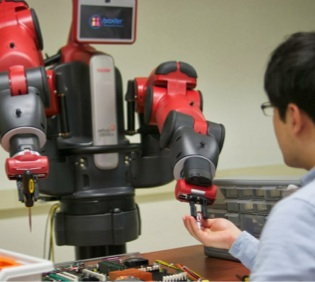
\includegraphics[scale=0.195]{figures/baxter_temp.jpg}%
  \caption{Placeholder for baxter results/image}
  \label{fig:baxter_results}
\end{figure}

% --- Options ---
\subsection{Options}

\begin{table}[H]
\centering
\begin{tabular}{ l || c c c c }
  State Space 		& None & Options & Affordances & Both 	 	\\ \hline
  \texttt{4rooms}  	& 	-		&	-	&	-	&	-	\\
  \texttt{Doors}  		& 	-		&	-	&	-	&	-	\\
  \texttt{Small}  		& 	-		&	-	&	-	&	-	\\
  \texttt{Medium}  	& 	-		&	-	&	-	&	-	\\
  \texttt{Large}  		& 	-		&	-	&	-	&	-	\\
\end{tabular}
\caption{Options vs. Affordances: CPU time per converged policy}
\label{table:minecraft_results_cpu}
\end{table}

% --- Minecraft ---
\subsection{Minecraft: Expert vs Learned vs None}

\dnote{We may want to make this a bar chart to include error bars more naturally. Since we want to include cpu time and bellman updates
for most results it might make sense to find a single chart type that can convey both (e.g. bar chart)}
\begin{table}[H]
\centering
\begin{tabular}{ l || c c c }
  State Space & No Affordances & Learned & Expert 	 	\\ \hline
  \texttt{Trench}  	& 	-		&	-	&	 -	\\
  \texttt{Mining}  	& 	-		&	-	&	-  \\
  \texttt{Smelting}  	& 	-		&	-	&	-  \\
  \texttt{Wall}  		& 	-		&	-	&	- \\
  \texttt{Tower}  		& 	-		&	-	&	- \\
\end{tabular}
\caption{Learned Affordance Results: Avg. Number of Bellman Updates per converged policy}
\label{table:minecraft_results_bellman}
\end{table}

\begin{table}[H]
\centering
\begin{tabular}{ l || c c c }
  State Space & No Affordances & Learned & Expert 	 	\\ \hline
  \texttt{Trench}  	& 	-		&	-	&	 -	\\
  \texttt{Mining}  	& 	-		&	-	&	-  \\
  \texttt{Smelting}  	& 	-		&	-	&	-  \\
  \texttt{Wall}  		& 	-		&	-	&	- \\
  \texttt{Tower}  		& 	-		&	-	&	- \\
\end{tabular}
\caption{Learned Affordance Results: CPU time per converged policy}
\label{table:minecraft_results_cpu}
\end{table}

\subsection{Minecraft: Learning rate}

\begin{figure}[H]
\centering
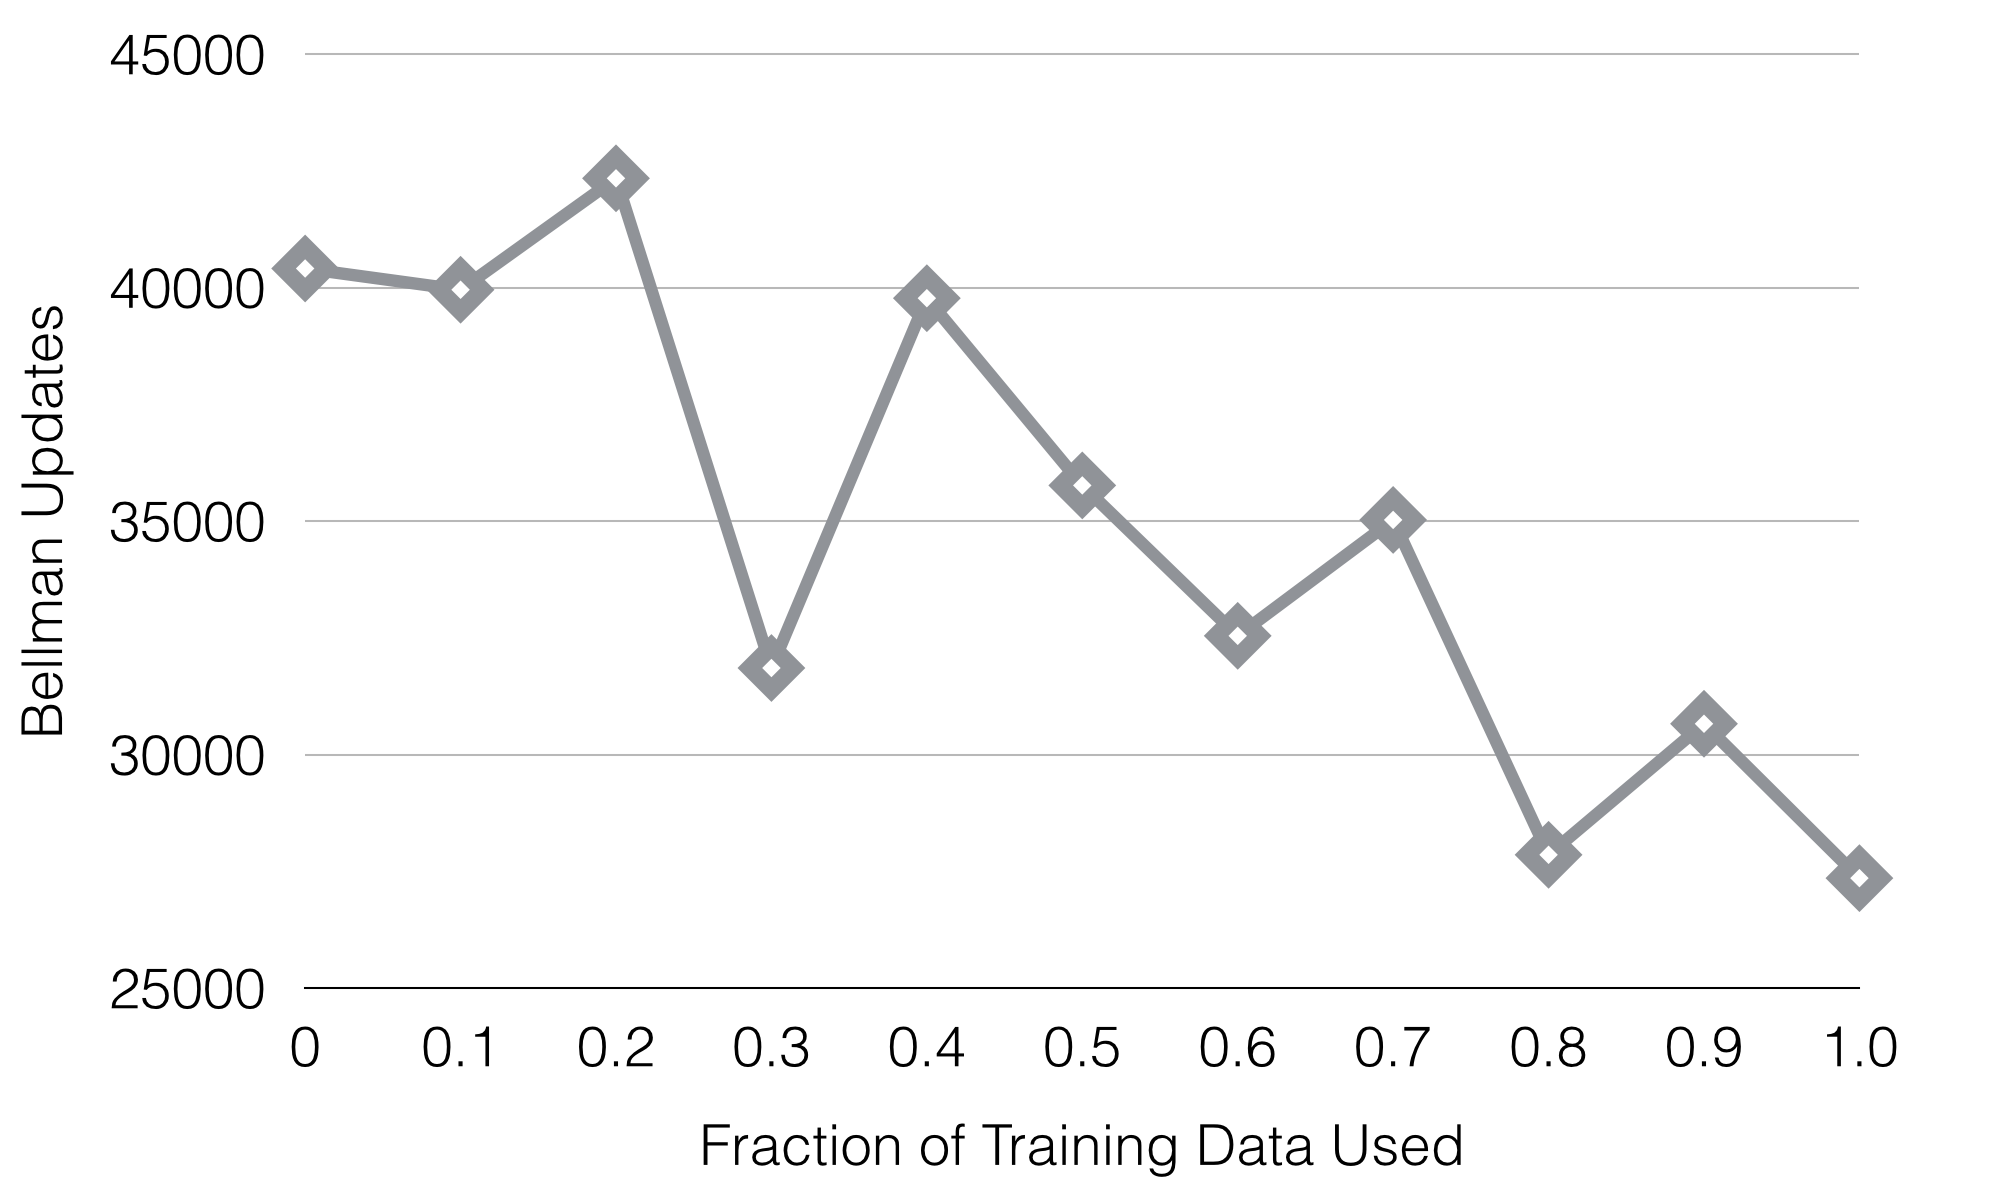
\includegraphics[scale=0.195]{figures/training_results.png}%
  \caption{Placeholder - will recollect this data given recent updates}
  \label{fig:training_results}
\end{figure}

% ====== Section: Conclusion ======
\section{Conclusion}
\label{sec:conclusion}

We proposed a novel approach to representing transferable knowledge in terms of
{\em affordances}~\cite{gibson77} that allows an agent to efficiently
prune its action space based on domain knowledge,
providing a significant reduction in the number of state-action pairs the
agent needs to evaluate in order to act optimally. We demonstrated the effectiveness of the affordance model by comparing a standard MDP solver
to its affordance-aware equivalent in a series of challenging planning tasks in the Minecraft
domain. Further, we designed a full learning process that allows an agent to autonomously learn useful affordances that may be used
across a variety of task types, reward functions, and state-spaces, allowing for convenient extensions to robotic applications.
We provided preliminary results indicating the effectiveness of the learned affordances, suggesting that
the agent may be able to discover novel affordance types and learn to tackle new types of problems on its own.

In the future, we hope to automatically discover useful subgoals - a topic of some active research \cite{Mcgovern01automaticdiscovery,Simsek:2005:IUS:1102351.1102454}. This will allow for affordances to reduce the size of the explored state-action space without requiring knowledge from an expert and increasing transferability across task types. Additionally, we hope to decrease the amount of knowledge given to the planner by implementing Incremental Feature Dependency Discovery ~\cite{ICML2011Geramifard_473}, which will allow our affordance learning algorithm to discover novel preconditions that will further enhance action pruning.


{\small
\bibliographystyle{plainnat}
\bibliography{main}
}
\end{document}


